\chapter{Web-Based Responsive Spoken Dialogue System}
\label{chap:web-based_responsive_spoken_dialogue_system}

\lettrine{I}{introduction} to this chapter\ldots

\pagebreak

\section{Architecture}
\label{sec:architecture_web-based}

\begin{figure}[t]
	\centering
	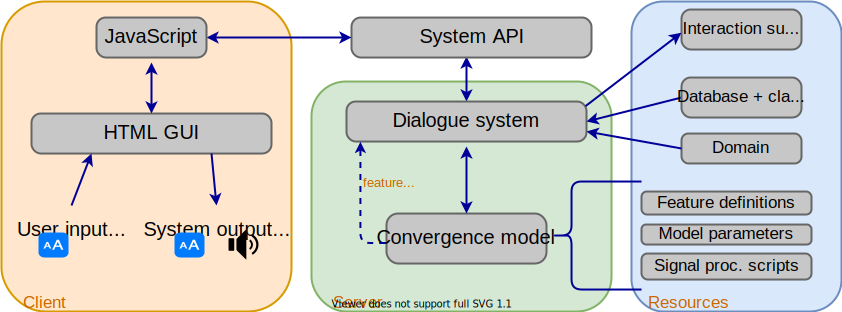
\includegraphics[width=\linewidth]{web-based_architecture_no-ajax}
	\caption[Architecture of a web-based responsive spoken dialogue system]
		{The architecture of the web-based responsive spoken dialogue system.
		The background colors distinguish between client components, server components, and customizable external resources.
		The dashed line indicates that the feature predictions may or may not be passed from the model to the system depending on the feature definition and update parameter.}
	\label{fig:web-based_architecture}
\end{figure}

For deepening the experimental possibilities and automating some aspects of the processes convergence-related experiments include, a dedicated systems with high degree of customizability was developed.
The system introduced tracks the states and changes of segment-level and suprasegmental-level phonetic features during a dialogue.
All of the analyses are automated and run in real-time, which not only saves a lot of time and manual work typically needed in convergence studies, but also makes the system more suitable for integration into other applications.
In \cref{sec:showcase} we demonstrate a possible use of the system by simulating a convergence study previously run entirely by hand.

% par about simulating
Simulating and triggering convergence on the phonetic level, as found in \ac{hhi}, may contribute a lot to the naturalness of the dialogue.
Our primary focus is on changes on the phonetic level, and more specifically variation in pronunciation and prosody, with no influence on the voice's overall acoustics.
\Acp{sds} with such personalized speech style may offer more natural and efficient interactions, as shown by \citet{Porzel2006entrainment}, and advance one more step away from the \emph{interface metaphor} \citep{Edlund2006twofaces} toward the \emph{human metaphor} \citep{Carlson2006humanlike}, which describe different user approaches when interacting with \ac{hci} systems.

% par about 

\putref{sds architecture}
\putref{computational model}
\putref{sds module}

\section{Background and related work}
\label{sec:background_and_related_work}

\ac{cat} \citep{Gallois2015CAT, Giles2007CAT, Shepard2001CAT} describes possible reasons for behavioral changes of interlocutors during interaction on various levels.
According to \citet{Weise2017towards}, integrating such changes into computer systems will enhanced \ac{hci} and provide improved tools for studying convergence in \ac{hci}.
\citet{Oviatt2004adaptive} discusses the advantages of systems that dynamically adapt their speech output to that of the user, and the challenges involved in developing and using these systems.

\section{System}
\label{sec:system}

The system introduced here is an end-to-end, web-based \ac{sds} with focus on phonetic convergence.
Besides placing convergence in the spotlight, it is designed to be flexible and to meet the researcher's needs by offering a wide range of component customizations (see \cref{subsec:models_and_cusomizations}).
Its online access via a web browser makes it scalable and simple for the end-user to operate.
The system's architecture and functionality are described in \cref{subsec:architecture},
its \ac{gui} and operation in \cref{subsec:graphical_user_interface},
and a real-world example of its utilization is demonstrated in \cref{sec:showcase}.

Ultimately, it offers a platform for studying and experimenting with phonetic convergence, with emphasis on the following:

\begin{description}
	\item[Focus~on~convergence] -- 
	offering an interface for general-purpose \acp{sds} with tools for analyzing and visualizing phonetic convergence.
	
	\item[Customizability] -- 
	allowing the user to experiment with different scenarios by configuring parameters and definitions in many of the system's components.
	
	\item[Online~scalability] -- 
	connecting multiple web clients to a server, allowing users to use it anywhere without installation, and helping experimenters to collect data remotely.
\end{description}

\subsection{Architecture}
\label{subsec:architecture}

As the system aims to offer a customizable playground for experimenting and studying phonetic convergence in \ac{hci}, a key aspect of its architecture is the separation between client-side, server-side, and external resources (see \cref{fig:web-based_architecture}).
This separation makes it possible to run multiple clients on different machines at the same time with a single server collecting the data from all of them at the same time.
The server, ideally located on dedicated machine, is operated by an a person responsible of designing and configuring the interactions, e.g., an experimenter.
It has an overview over all of the interactions with the system and collects all of the audio recordings, analyses, and any other data in one place.
This separation of the server grants the experimenter a lot of freedom and flexibility, since resources like feature configurations and dialogue domain can be modified independently of specific machines interacting with the system.
These changes are transparent to the users, and no effort is required from them aside from restarting the interaction to apply them.
As the server is also responsible for the connection to the client, it is also possible to defined different configuration to different users based on some characteristics, like their gender, native language, phonetic preferences etc.
This flexibility makes it easier and quicker to create new scenarios of interaction and to experiment with different features and parameters, without the need to create a dedicated system for each experiment.

In addition to the technical advantages, letting users interact with the system on a separate machine broadens the usage possibilities.
For example, an experiment can be carried out remotely, without the need to invite participants to the recording studio one by one.
Furthermore, as the connection to the server is done via a web browser, participants can connect use the system with their own computers wherever and whenever it suits them, without any additional installation or technical configurations.
And most importantly, multiple users can connect to the system simultaneously.
All of these makes it possible to collect data from many users rapidly and easily.

\subsubsection{Dialogue System}
\label{subsubsec:dialogue_system}

The \emph{Dialogue System} component is the core of the system (see \cref{fig:web-based_architecture}).
It controls the flow of the interaction, processes the user's input, and generates the system's responses.
As shown in \cref{fig:adaptation_module_architecture}, it consists of typical \ac{sds} components such as \ac{nlu} and a \ac{dm}, but contains an \ac{asp} module as well \citep{Raveh2017SemDial}.
This module is responsible for processing the audio\footnote{\label{foot:praatver}using Praat, v6.0.35, \url{http://praat.org/}, \citep{Boersma2018praat} as the signal processing back-end} and extracts the features required by the convergence model (\cref{subsubsec:convergence_model}).
While the \ac{nlu} component uses merely the transcription provided by the \ac{asr}, the \ac{asp} module analyzes the speech signal itself.
More specifically, it tracks occurrences of the defined features and passes the measured values to the convergence model, as explained in \cref{subsubsec:tracked_features}, which, in turn, forwards the tracked feature parameters to the \ac{tts} synthesis component.
Finally, the \ac{tts} engine takes the text generated by the \ac{nlg} component, and, if phonetic-level manipulation is supported, synthesizes the utterance using the values specified by the convergence model.
The \emph{OpenDial} dialogue framework \citep{Lison2016opendial} is used in the \ac{sds} component of the system.
The \ac{asr} module uses CMUSphinx \citep{Lamere2003sphinx} with additional customized functionality required for the \ac{asp} module, and the \ac{tts} is driven by MaryTTS \citep{LeMaguer2017uprooted, Schroeder2003mary}.
The rule-based implementation of the \ac{nlu} and \ac{nlg} modules is described in \cref{subsubsec:dialogue_domain}.

\subsection{Models and customizations}
\label{subsec:models_and_cusomizations}

The system aims to offer a platform for \acp{sds} with convergence support that can be modified and customized according to the user's needs.
All of the aforementioned system components can be customized to some extent.
This also includes the phonetic convergence model, the features tracked by the system, and the dialogue domain.

\subsubsection{Convergence model}
\label{subsubsec:convergence_model}

The computational model for phonetic convergence used in our system is derived from the one introduced in \citet{Raveh2017Interspeech}.
Different behavioral patterns with respect to phonetic convergence that were observed in \ac{hhi} and \ac{hci} experiments \citep{Cohen2017converging, Gessinger2017Interspeech, Schweitzer2016exemplar, Babel2010dialect} can be simulated by combinations of the model's parameters presented in \cref{tab:comp_model_parameters}.
For example, the parameter \emph{allowed range} describes the segments that would be perceived as instances of a feature by the interlocutor.
The number of instances of a feature which the interlocutor can hold in his or her short-term memory is defined by the parameter \emph{history size} (or \emph{exemplar pool size}).
Similarly, the parameter \emph{convergence rate} determines how quickly the system converges to the human interlocutor with respect to the tracked features.
This comes to characterize the sensitivity of a speaker to other pronunciation variants.
\emph{Calculation method} specifies how the feature's new value is obtained from the instances in the exemplar pool.
This can be a simple average, some smoothing function, or any other function defined by the user.
All of the model's parameters can be modified in the configuration file.
The responsiveness algorithm's pipeline is summarized in \cref{fig:adaptation_module_pipeline} and is described in detail in \citet{Raveh2017Interspeech}.
\todo{here create an algorithm block version of the figure to not repeat it twice}

\subsubsection{Tracked features}
\label{subsubsec:tracked_features}

\todo[inline]{this section (and maybe other parts in this chapter are pretty much redundant to the pipeline implementation in the module chapter. make sure such parts are removed and refer to the relevant place there.)}

The entire convergence process is based on the phonetic features that are defined as \enquote{convergeable}, i.e., phonetic features that are prone to variation, and is triggered whenever the \ac{asr} component detects a segment containing a phoneme associated with one or more of these features.
These feature definitions aim to capture phonological rules.
For instance, the German phonological \textipa{/@/} elision rule in word-final syllables $\langle$-en$\rangle$ is defined by \citep[adapted from][pp.\,142--143]{Benware1986phonetics}
%
\begin{equation}
\text{\textipa{@n}}\longrightarrow \varnothing \text{\textipa{\s{n}}} \diagup
%	\left[\text{$-$son}\right] \ \_\_ \ \{\text{\#}, \left[\text{+const}\right]\} .
\text{+consonantal} \ \_\_ \ \ \text{\#} .
\label{eq:elision_rule}
\end{equation}
\eqname{Rule implementation: Schwa elision in German}
%
Each feature is represented by a key-value map of parameters in the editable configuration file.
The target phoneme (here \textipa{/@/}) is defined in the feature definition's \emph{phoneme} key in the configuration file.
However, merely defining the target phoneme is not enough, because the rule should only be triggered in the context specified on its right-hand side.
This is done using the \emph{context} parameter.
%Finally, since the target feature definitions are simply machine-readable phoneme sequences, it is easy to define new features -- even in another language (provided a phoneme-emitting \ac{asr} component for that language is available).
As an example, the parameter map of the feature \textipa{[E:]}~vs.~\textipa{[e:]} might look as follows:

\begin{description}[labelindent=1.5cm, labelwidth=\widthof{\quad \bfseries calculation}]
	\item[name]	ee\_E
	\item[phoneme] EHH
	\item[context] .* EHH .*
	\item[initial] 451, 2116, 2763
	\item[minimum] 300, 1500, 2500
	\item[maximum] 750, 2900, 4800
	\item[measure] formants
	\item[calculation] decaying average
	\item[sensitivity] 0.3
\end{description}
%
The value of the key \emph{measure} is \enquote{formants}, which means that this feature is evaluated by the segment's formant values (as specified in the corresponding signal processing script).
The values of the \emph{minimum} and \emph{maximum} keys stand for the acceptable value range for this feature.
This avoids distorted values due to \ac{asr} error and lets the user put their phonetic expertise to use.
\todo{what?}
In this case, the three values of these keys set the first three formant frequencies.
Furthermore, the initial value of this feature in the model is also specified in the \emph{initial} key.
This determines the variation of the feature with which the model starts.
In this example, the convergence rate (\emph{sensitivity} key) is set to 0.3, and the \emph{calculation} method, to \enquote{decaying average}, which is a recursive weighted average measure defined as,
%
\begin{equation} 
\label{eq:decaying_average} 
\mu_n = \frac{1}{n}\sum_{i = 2}^{n}(\eta v_i + (1 - \eta )\mu_{i-1}), 
\end{equation} 
\eqname{Decaying average}
%
where $n$ is the number of exemplars in memory, $\eta$ is the decay rate (here, 0.5), $\mu_{i-1}$ is the accumulated decaying average from the previous exemplar, and $v_i$ is the value of the $i$-th exemplar. 

Since the system's main focus is on phonetic convergence, it is essential to also provide useful information regarding the realizations of the tracked features.
To that end, a classifier can be associated with each feature to provide real-time predictions for both the user's and the system's realizations of that features, as demonstrated in \cref{fig:plot}.
With this information available, more meaningful insights can be gained into the variation dynamics in the dialogue.

\subsubsection{Dialogue domain}
\label{subsubsec:dialogue_domain}

The dialogue's flow is specified in \emph{OpenDial}'s \citep{Lison2015developing} XML-based format\footnote{\url{http://www.opendial-toolkit.net/user-manual/dialogue-domains}}.
%This format offers a structure for building models, rules, and conditions, which define the dialogue script.
Additional parameters are introduced for triggering models or rules, or for processing by external modules of the \ac{sds}, as in the case of the \ac{asp} module.
%More details on how to build a domain file can be found in \citet{Lison/Kennington:2015}.
The format of the domain file makes it easy to define new scenarios for the system,
such as a task-specific dialogue, general-purpose chat, or an experimental setup.

\subsubsection{Speech processing}
\label{subsubsec:speech_processing}

Multiple components of the system deal with different aspects of speech processing.
The \ac{asr} component uses CMUSphinx\footnote{Sphinx4 version 5prealpha, \url{https://cmusphinx.github.io/}} \citep{Lamere2003sphinx}.
The acoustic model and pronunciation dictionary were taken from CMUSphinx models on SourceForge\footnote{\url{https://sourceforge.net/projects/cmusphinx/files/Acoustic\%20and\%20Language\%20Models/German/}}, and a customized language model was created with SRILM \citep{Stolcke2002SRILM}).
All of the phonetic analysis is done using Praat \citep{Boersma2018praat}.
MaryTTS \citep{LeMaguer2017uprooted} is used as the \ac{tts} engine, with \emph{bits1-hsmm} and \emph{bits3-hsmm} for female and male voices, respectively.

\subsection{\Acl{gui}}
\label{subsec:graphical_user_interface}

The interaction of the user with the system is done via a web-based \ac{gui}.
This \ac{gui} consists of a navigation bar and four areas:
a chat area, where the dialogue is shown (see \cref{subsubsec:chat_area}),
an interaction area where the user input is recorded (see \cref{subsubsec:interaction_area}),
a graph area where the tracked features are visualized and analyzed (see \cref{subsubsec:graph_area}),
and a notification area where prompts for the user can be shown.

\subsubsection{Chat area}
\label{subsubsec:chat_area}

\begin{figure}[t]
	\centering
	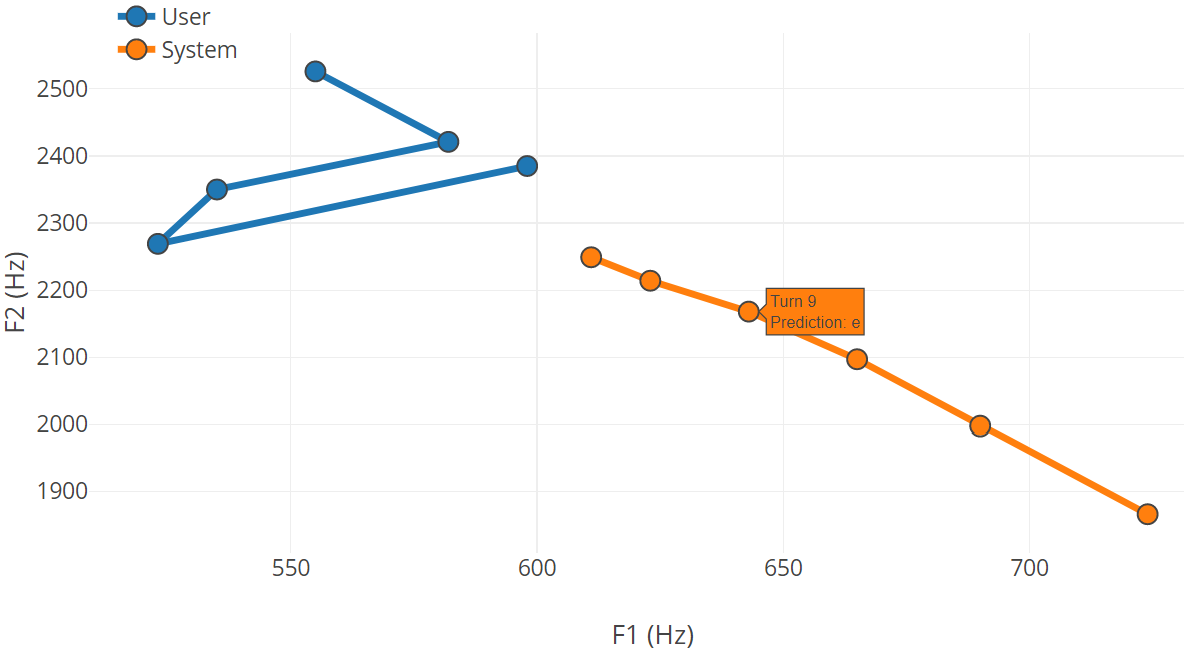
\includegraphics[width=\linewidth]{plot_area}
	\caption[Real-time visualization of phonetic changes]{A screenshot of the plot area showing the states of the feature \textipa{[E:]}~vs.~\textipa{[e:]} during an interaction.
		The system's internal convergence model (orange, bottom right) gradually adapts to the user's (blue, upper left) detected realizations.
		A prediction of the feature's current realization is given for both interlocutors.
		The text box annotates a turn in which the system's realization changes.}
	\label{fig:plot}
	\todo[inline]{make a better screenshot of this area, maybe also with more interesting interactions}
\end{figure}

The interaction between the user and the system is shown in a chat-like representation (see example in \cref{app:dialogue_example}).
Each turn's utterance appears inside a chat bubble with different colors for the user and the system.
The turns are also numbered, to better track the dialogue progress and analysis shown in the plots in the graph area.
The history of the chat is kept under the \emph{Turns} drop-down in the navigation bar, and it is possible to reset the interaction to start a new session.
%Beside the chat bubbles, the system can also insert general-purpose messages to the users, which are not part of the dialogue's flow.

\subsubsection{Interaction area}
\label{subsubsec:interaction_area}

The user can interact with the system with written or spoken input using the controls in this area.
Text-based interactions progress through the dialogue (if applicable) and trigger any subsequent domain model, but will not affect convergence-related models, since there is no audio input to process.
Spoken input can be provided either by speaking into the microphone or via audio files with pre-recorded speech.
The latter option is especially useful for simulating specific user input, or for reproducing a previous experiment with the exact same input, as done in \cref{subsec:validation}.

\subsubsection{Graph area}
\label{subsubsec:graph_area}

Each of the tracked features is visualized in a separate plot, and new datapoints are automatically added whenever applicable.
These plots are generated using the Plotly library\footnote{\url{https://plot.ly}}, which provides some interactive functionalities.
For example, hovering over a datapoint in a graph reveals additional information, such as the turn in which it was added, or the realized variant of the feature produced in that turn as predicted by its classifier.
\Cref{fig:plot} shows a graph with several accumulated datapoints.

%\subsubsection{Settings and help}
%\label{subsubsec:settings_and_help}
%
%An additional modal window can be called, in which various settings can be changed, and some usage information is provided.
%Configurable settings include the convergence model parameters, domain file, \ac{gui} tweaks, and more.
%These settings can be modified at any point during the interaction, so that it is possible to experiment with different configurations in real-time.
%For persistent changes, it is also possible to edit the configuration file itself, which is loaded when the system starts.
%The usage tab explains the various functionalities of the system and how each area of the \ac{gui} works.
%It also lists special commands that can be executed from text field (used for simulating the user's input, as mentioned in \cref{subsubsec:interaction_area}).
%These commands include printing a short or detailed summary of the phonetic changes throughout the interaction, extracting the data from the features' plots (e.g., for further analysis), and more.
%\todo{screenshot with the settings tab}

\section{Showcase: simulating a shadowing experiment}
\label{sec:showcase}

To demonstrate the capabilities of the system, we utilized it to replicate a convergence experiment.
For that, the shadowing experiment carried out by \citet{Gessinger2017Interspeech} was chosen.
The experiment is designed to trigger and analyze phonetic convergence by confronting the participants with stimuli, in which certain phonetic features are realized in a way different from their own.

For this simulation, the original stimuli and participants' utterances were used.
However, all of the analyses that were done ex post facto, and to some extent manually, in the original experiment, like detecting the realized variant, measuring the features, etc., are done automatically in the simulated experiment.
This results in an automated, reproducible execution, and also offers additional insights via classification of feature realizations and dynamic visualizations in the web \ac{gui}.
Finally, using the system, the experiments becomes dialogue-based, which enhances its \ac{hci} nature.

\subsection{Target features and stimuli}
\label{subsec:target_features_and_stimuli}

The experiment deals with three segment-level phonetic features that show variation across native speakers of German:

\begin{description}[labelindent=1.3cm, labelwidth=\widthof{\quad \textipa{[I\c{c}]}~vs.~\textipa{[Ik]}}]
	\item [\textipa{[E:]}~vs.~\textipa{[e:]}] in word-medial $\langle$ä$\rangle$
	\item [\textipa{[I\c{c}]}~vs.~\textipa{[Ik]}] in word-final $\langle$-ig$\rangle$
	\item [\textipa{[\s{n}]}~vs.~\textipa{[@n]}] in word-final $\langle$-en$\rangle$
\end{description}

\noindent
Although these feature may pass as light dialectical markers \citep{Mitterer2013regional}, they do not carry any difference in meaning, and are generally ascribed to personal preference of speaking style.

The experiment's stimuli consist of these features embedded into 15 short carrier sentences (see examples in \cref{tab:target_features}) and 25 filler sentences, in which none of the features occur.
Although the features' underlying values are gradual, they are perceived as two-way categorical variations.
To map these underlying values to a specific variant, the system associates a classifier with each feature, as explained in \cref{subsec:training_and_classification}.

\begin{table}[t]
	\centering
	\begin{tabularx}{\linewidth}{@{}*{5}{l}}
		\toprule
		
		War          	& das          			& Ger\textbf{\underline{ä}}t	& sehr          	& teuer? \\
		\emph{Was} 		& \emph{the} 			& \emph{device}           		& \emph{very} 		& \emph{expensive?} \\[0.1cm]
		
		Ich          	& bin         			& sücht\textbf{\underline{ig}}	& nach				& Schokolade. \\
		\emph{I}   		& \emph{am} 			& \emph{addicted}				& \emph{to} 		& \emph{chocolate.} \\[0.1cm]
		
		Wir         	& besuch\textbf{\underline{en}} 						& euch				& bald          & wieder. \\
		\emph{We} 		& \emph{will visit}		& \emph{you} 					& \emph{soon} 		& \emph{again.} \\
		
		\bottomrule
	\end{tabularx}
	\caption[Example sentence for selected phonetic features]{Examples of stimuli containing the target features. Each stimulus contains only one feature.}
	\label{tab:target_features}
\end{table}

\subsection{Experimental procedure}
\label{subsec:experimental_procedure}

Only those parts of the experiment are explained here that are relevant to its simulation in the dialogue system.
For validation purposes, the experimental procedure stayed as faithful as possible to the procedure of the original experiment, even though more aspects of it could be automated.
The entire experimental procedure, as well as more information regarding its setup, is detailed in \citet{Gessinger2017Interspeech}.

The experiment consists of three phases: \emph{baseline} production, \emph{shadowing} task, and \emph{post} production (see \cref{fig:HCIConvFlow}).
In the \emph{baseline} phase, the participants were asked to read out the stimuli from a monitor.
The participant's most frequent variant in this phase is configured into the system.
Then, in the \emph{shadowing} task, the participants produced the stimuli sequentially, each after listening to another voice (either natural or synthetic, both male and female) producing the opposite category of the relevant target feature.
Based on the production in this phase, the participant's tendency, pace, and degree of convergence were analyzed.
Finally, in the \emph{post} phase, the participant once again read out the stimuli from a screen.
The purpose of this phase was to examine whether any convergence remained in effect even in the absence of non-preferred input.
A shortened example of the shadowing phase's flow is shown in \cref{app:dialogue_example}.

\subsection{Training and classification}
\label{subsec:training_and_classification}

The validation stays faithful to the original experiment in every possible aspect.
Therefore, the training data used for each classifier contains only the productions of the corresponding target feature from a single stimulus set, since these are the productions to which the participants were exposed during the experiment.
This provides relatively few -- but at the same time very precise -- datapoints for each classifier,
which were obtained using the same signal processing technique as the data collected in the experiment.
The classifiers were trained offline on these datapoints.
However, the system also supports incremental, online re-training whenever requested by the user,
such as, every time the convergence model is updated.

A \ac{smo} \citep{Platt1999fast, Platt1998sequential} implementation of the \ac{svm} classifier \citep{Vapnik1998support} was using for training.
Depending on the target feature, this may also be a multivariate \ac{svm} classification \citep[e.g.,][]{Joachims2005support}.
Each turn's predictions, as well as other details, are added as interactive annotations to the dynamic graph of the relevant features, as shown in \cref{fig:plot}.

\subsection{Validation}
\label{subsec:validation}

\begin{figure}[t]
	\centering
%	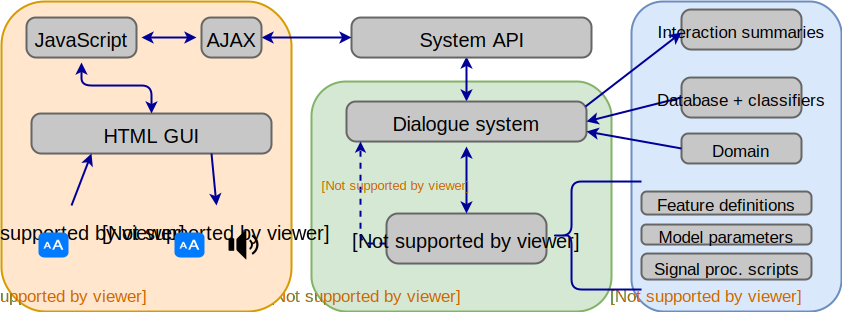
\includegraphics[width=\linewidth]{web-based_architecture}
	\missingfigure{bull's eye figure and bars figure}
	\caption[]
		{}
	\label{fig:validation}
\end{figure}

We simulated the shadowing experiment by configuring the domain file with a definition of the transition between the phases, as well as the flow within each phase.
This automates the procedure and adapts it to the participant's pace.
Additional variables are defined and handled as well, helping the system to track the experiment's flow and state.
Participants were simulated by using their recorded speech from the original experiment.
After each turn, any relevant \ac{sds} module was triggered based on the simulated participant's input.
The stimulus order from the original experiment was preserved.
Since the \emph{post} phase is effectively the same as the \emph{baseline} phase, it was considered redundant and excluded from the simulation.
In this section, we focus on the validation for the feature \textipa{[E:]}~vs.~\textipa{[e:]} as a representative example for the phonetic adaptation capability of the system.

For the baseline phase, the validation examined the degree to which the underlying convergence model accumulated enough data to adopt the user's variant of the feature.
Stronger and quicker adoption indicates a more stable and precise preferred variant of the participant.
The user's and model's preferred variants were determined based on the majority vote at the end of this phase.
For example, if the user realized one variant twice and another three times, the latter is considered to be preferred.
\Cref{tab:validation_baseline} shows the degree of the model's adoption of the user's preferred variant, according to their majority votes, using different values of the \emph{sensitivity} parameter.
Interestingly, higher values do not necessarily result in higher percentages.
The value 0.3 provided the highest results, and was therefore used through the rest of the simulation.

\begin{table}[t]
	\centering
	\begin{tabularx}{\linewidth}{X*{4}{S[table-format=2.1]}}
		\toprule
		sensitivity (\numrange{0}{1}) &  0.2 &  0.3 &  0.4 &  0.5 \\
		adoption (\si{\percent})      & 79   & 86   & 75   & 69   \\
		\bottomrule
	\end{tabularx}
	\caption{Model's convergence coverage with different parameters.}
	\label{tab:validation_baseline}
\end{table}

After obtaining the preference of each participant, the degree of convergence was examined per utterance in the shadowing phase.
The participants were grouped based on their convergence behavior:
One group of participants showing low to no tendency to converge (\SI{\le 10}{\percent} of their utterances),
the second, with varying degrees of convergence (\SIrange{10}{90}{\percent}),
and a third group of participants who were very sensitive to the stimuli's variation (\SI{\ge 90}{\percent} of their utterances).
We refer to these groups as \emph{Low} (\SI{23}{\percent} of participants), \emph{Mid} (\SI{50}{\percent}), and \emph{High} (\SI{27}{\percent}), respectively.
The feature's classifier was determined on the fly, so that the prediction for each utterance was decided based on the stimulus type to which the participant was listening (e.g., a classifier trained on synthetic stimuli was used for participants listening to such stimuli).

For the purpose of the validation, we regard the shadowing phase as an annotation task of the realized variation in the utterances.
The three annotation sets are the stimuli themselves (\emph{Stim}), the system's online classification of the participants' production (\emph{Sys}), and the labels obtained as additional references for the participants' productions (\emph{Ref}).
Note that \SI{100}{\percent} would mean complete convergence to every stimulus, which cannot be reasonably expected \citep[cf.][]{Gessinger2017Interspeech}.
The same holds for the Cohen's kappa ($\kappa$) values\footnote{as calculated by the \emph{kappa2} command of the \emph{irr} R package, v0.84, \url{https://cran.r-project.org/package=irr}}, which are expected to be lower for \emph{Low}, as a lower degree of convergence was found among these participants.
As \cref{tab:validation_shadow_similarity} shows, convergence was found in \SI{48}{\percent} of the utterances for \emph{Sys-Stim} and \emph{Ref-Stim}.
However, the \emph{Ref-Sys} similarity is only \SI{66}{\percent}, which means that convergence was found in different instances.
The $\kappa$ values in \cref{tab:validation_shadow_kappa} give an additional view on these results.
The \emph{Ref-Sys} agreement is around 0.2 (fair agreement) for \emph{Mid}, but much lower for the other two groups,
confirming that more differences are expected to be found between \emph{Sys-Stim} and \emph{Ref-Stim} in the \emph{Low} and \emph{High} groups.
Moreover, \emph{Sys-Stim} shows greater variation of $\kappa$ values across the three groups, indicating higher separation between the three categories of convergence behavior.
This provides a more meaningful overview of the participants' convergence patterns.
% kappa itepratation classes taken from http://www.statisticshowto.com/cohens-kappa-statistic/

\section{Conclusion and future work}
\label{sec:conclusion}

We have introduced a \acf{sds} with phonetic convergence capabilities.
The system is able to track the state of configured phonetic features and change its \acf{tts} output accordingly, based on an internal convergence model.
This combines work done in the fields of phonetic convergence and adaptive \acp{sds}.
Many aspects of the system are customizable, which makes it flexible in terms of possible supported scenarios.
This includes multiple parameters defining the target phonetic features, which allows experimentation with different features.
The system can run on a separate server, which makes it easier to scale its use.

In addition, we replicated a shadowing experiment, which examined phonetic convergence regarding certain features, showcasing the \ac{sds}'s performance and simulation capabilities.
Running the experiment in this way not only saved time by automating the annotation and phonetic analysis, but also offered additional insight such as visualization and on-the-fly classification.

By validating the system in this way, we are confident that phonetic convergence can be studied using our \ac{sds} in a more objective way, focused on \ac{hci}.
We firmly believe that this is one step forward toward personalized, phonetically aware \acp{sds}, which are likely to enable more natural and efficient interaction.

\begin{table}[t]
	\centering
		\begin{tabularx}{\linewidth}{X*{3}{S[table-format=2.0]}}
			\toprule
			Group & {\emph{Sys}-\emph{Stim}} & {\emph{Ref}-\emph{Stim}} & {\emph{Ref}-\emph{Sys}} \\
			\midrule
			\emph{Low}  & {<1} &  7 & 16 \\
			\emph{Mid}  &  22  & 23 & 32 \\
			\emph{High} &  26  & 18 & 18 \\
			All   		&  48  & 48 & 66 \\
			\bottomrule
		\end{tabularx}
%		\caption{Similarity (\si{\percent})}
		\label{tab:validation_shadow_similarity}
\end{table}
\begin{table}
		\begin{tabularx}{\linewidth}{X*{3}{S[table-format=2.2]}@{\quad}}
			\toprule
			Group & {\emph{Sys}-\emph{Stim}} & {\emph{Ref}-\emph{Stim}} & {\emph{Ref}-\emph{Sys}} \\
			\midrule
			\emph{Low}  & -0.57*** & -0.08   & 0.17    \\
			\emph{Mid}  & -0.15*   & -0.15*  & 0.27*** \\
			\emph{High} &  0.81*** & -0.04   & 0.03    \\
			All   		& -0.11*   & -0.13** & 0.21*** \\
			\bottomrule
		\end{tabularx}
%		\caption{Agreement (Cohen's $\kappa$).
%			\enquote*{*} means $p$~value $<0.05$, \enquote*{**} means $p$~value $<0.005$, and \enquote*{***} means $p$~value $<0.0005$}
		\label{tab:validation_shadow_kappa}
	\caption[Similarity and agreement evaluation of system and stimulus sets]{A summary of the similarity and agreement between the system's (\emph{Sys}), references (\emph{Ref}), and stimuli (\emph{Stim}) annotations of the shadowing phase productions.}
	\label{tab:validation_shadow}
\end{table}
	\todo{somehow combine these tables. or maybe replace it with a better analysis}

Future work will pursue two independent directions:
regarding phonetic convergence, supporting more features will make the system more comprehensive and useful for studying a wider range of phenomena.
Specifically, adding support for supra-segmental (i.e., prosodic) features will enable replication of experiments similar to, e.g., \citet{Levitan2014acoustic, Levitan2016implementing} in the same manner as in \cref{sec:showcase}.

Regarding user acceptance, it would be interesting to examine whether users show any preference toward an \ac{sds} that converges to their speech on the phonetic level, and whether they would change their speaking style based on the system's output, forming an interaction with mutual and dynamic convergence.
The first research question can be tested by comparing user interaction with a baseline system and one with convergence capabilities, and evaluating the users' performance and satisfaction.
The second research question can be investigated by comparing the users' speech when interacting with either system configuration.
Additionally, to test the system's influence on users' speech, the users can train with an intelligent \acf{call} or \acf{capt} system, which will change its learner model based on their input.
Task completion rate, performance accuracy, and completion time metrics can be used to evaluate how helpful the system is.

\begin{figure}[h!]
	\centering
	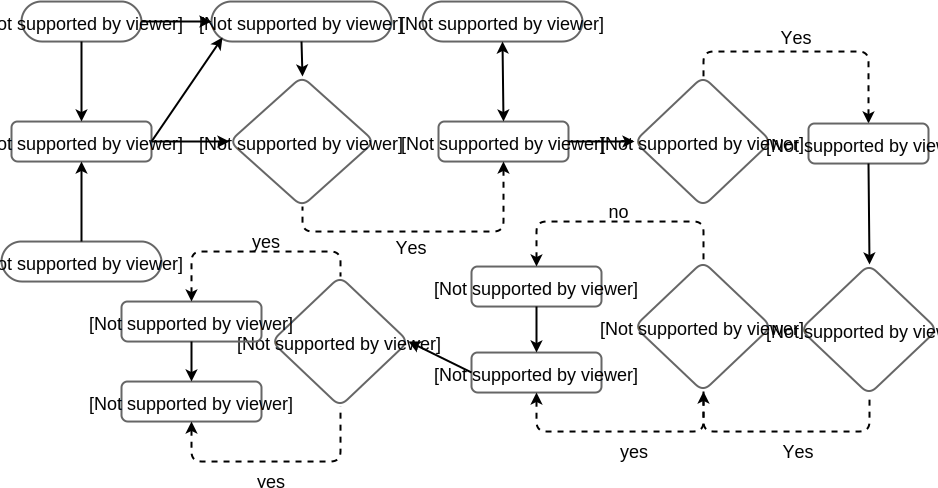
\includegraphics[width=\linewidth]{pipeline}
	\caption[Phonetic convergence algorithm pipeline]{Overview of the phonetic convergence pipeline used in the computational model.
		Rectangles represent steps where an action is performed, round rectangles are inputs (either for external resources or from the system), and diamonds stand for decision points.
		When a decision node does not have a \enquote{no} outcome it means that the process is terminated (and therefore no convergence occurs) if the condition is not met.
		The pipeline can only be successfully completed at the \enquote{Set feature's new value} node.
		However, if the \enquote{Add exemplar} action was performed prior to termination, the exemplar is not removed and will be taken into consideration the next time the pipeline is triggered for the feature with which it is associated.
		The \enquote{feature definitions} come from the configuration file and can be changed by the user.}
	\label{fig:adaptation_module_pipeline}
\end{figure}

\todo{fix in figure: two ``yes''es are going out of the Convergence Limited block}

\todo{use colors to associate each shape (excluding arrows) to a step in the pipeline (maybe same colors as in stripes figure?)}

\todo[inline]{somewhere in the thesis where evaluation of an actual system is discussed, talk in detail about the challenge that there is no absolute correct answer regarding how and how much to converge (user dependent, etc.) and for the same reasons there is no gold standard to compare against. so need to find other criteria for evaluation.}

\section{Dialogue example}
\label{app:dialogue_example}
\todo{Put a relevant and interesting chat example (if that's even necessary here)}
%\begin{figure}[h!]
%	\centering
%	\adjustbox{max width=\linewidth}{\begin{tikzpicture}
\matrix (m) [%
  matrix of nodes,
  inner sep=1ex,
  row sep=-1.5ex,
  column sep=1ex,
  every node/.style={%
    text width=18em,
    text depth=0.5ex,
    rectangle callout,
    callout pointer width=5,
    rounded corners,
    fill,
    text=white
  },
  column 1/.style={%
    callout relative pointer={(-1,0)},
    fill=orange,
    align=left
  },
  column 2/.style={%
    callout relative pointer={(1,0)},
    fill=blue,
    align=right
  }
]{%
  Hallo! Bist du bereit? & \\
  & ja \\
  Die Bestätigung ist für Tanja & \\
  & die bestätigung ist für tanja \\
  War das Gerät sehr teuer? & \\
  & war das gerät sehr teuer \\
  Ich mag die Qualität deiner Tasche &\\
  & ich mag die qualität deiner tasche \\
  Der Schädling sieht aber komisch aus & \\
  & der schädling sieht aber komisch aus \\
  Wie viel Verspätung hat der Zug? & \\
  & wie viel verspätung hat der zug \\
  Vielen Dank, das war alles & \\
};
\begin{scope}[%
  every node/.style={%
    rounded corners,
    fill=gray,
    text=white,
    outer sep=1ex
  }
]
\foreach \y in {1,3,...,13} {%
  \node [anchor=east] at (m-\y-1.east) {\y};
}
\foreach \y in {2,4,...,12} {%
  \node [anchor=west] at (m-\y-2.west) {\y};
}
\end{scope}
\end{tikzpicture}
}
%	\caption{An illustration of the chat area at the end of the shadowing task.
%		The sentences shown here are the subset of sentences containing the feature \textipa{[E:]}~vs.~\textipa{[e:]}.
%		User utterances are in blue, the system's are in orange.
%		The interaction starts with the system asking the user whether he is read, where only a \enquote{yes} will progress forward.
%		The user then repeats the sentences presented by the system, until the system declares that there are no sentences left.
%		Each utterance is labeled with the turn number it appeared in.
%		This numbering can be used to track the analysis of this turn, as shown in \cref{fig:plot}.}
%	\label{fig:chat_example}
%\end{figure}
